\chapter{基本概念}
\label{ch:rl-basic}

% ════════════════════════════════════════════════════════════════
%  来源：赵世钰《强化学习的数学原理》第 1 章（源页 p023–p035，逐页核对）。
%  原原本本忠实转写：保留全部正文 / 公式 / 推导 / 表 / 示例 / 图注 / 问答。
%  插图分层：
%    图 1.1（本章在全书中的位置导航图）弃用，留 %TODO，不收录；
%    图 1.2 网格世界、图 1.3(a) 状态网格、图 1.7 抽象成马尔可夫过程 → TikZ 重绘；
%    图 1.3(b) 动作、图 1.4(a)(b) 确定性策略与轨迹、图 1.5 随机策略、
%    图 1.6(a)(b) 两策略及轨迹 → 含密集箭头/示意，用 \includegraphics。
% ════════════════════════════════════════════════════════════════

% TODO: 图 1.1「本章在全书中的位置」(Zhao 导航图) 弃用，不收录。
%       源 MD: images/de7df7384e5bd53fcf1763f6e1d209b9c4eeb23e0f6c066667f85611e61dd064.jpg

本章介绍强化学习中最基本的概念，这些概念将在本书中广泛使用。本章首先通过网格世界的例子引出这些概念，之后会在马尔可夫决策过程的框架中对它们进行更加正式的介绍。

% ════════════════════════════════════════════════════════════════
\section{网格世界例子}
\label{sec:rl-basic-grid-world}

\cref{fig:rl-basic-grid-world} 展示了一个网格世界（grid world）的例子。其中有一个智能体（agent）在网格中移动。在每个时刻，智能体只能占据一个单元格。白色单元格代表可以进入的区域，橙色单元格代表禁止进入的区域，蓝色单元格代表目标区域。智能体的任务是从一个初始区域出发，最终到达目标区域。这个网格世界的例子非常直观，能够很好地解释许多新概念、新算法，将在本书中广泛使用。

\begin{figure}[ht]
\centering
\begin{tikzpicture}[scale=0.9, >=Stealth,
  cell/.style={draw, minimum size=16mm, inner sep=0pt},
  forb/.style={cell, fill=second!22},
  targ/.style={cell, fill=main!18}]
% 3x3 网格世界（与源图 1.2 一致）：白色=可进入，橙色=禁止区，蓝色=目标区
% 坐标 (x,y)：左上为 s1，右下为 s9（y 向下递减）
\foreach \x in {0,1,2}{
  \foreach \y in {0,1,2}{
    \node[cell] at (\x,\y) {};
  }
}
% 禁止区（橙）：s6（右中）与 s7（左下）
\node[forb] at (2,1) {\footnotesize 禁止};
\node[forb] at (0,0) {\footnotesize 禁止};
% 目标区（蓝）：s9（右下角）
\node[targ] at (2,0) {\footnotesize 目标};
% 出发区（左上 s1）
\node at (0,2) {\footnotesize 出发};
% 智能体示意（中心 s5）
\node[circle, fill=black, inner sep=1.6pt] at (1,1) {};
% 从出发到目标的示意路径（虚线）
\draw[dashed, gray!70] (0,2) -- (1,2) -- (1,0) -- (2,0);
\end{tikzpicture}
\caption{网格世界的示例。}
\label{fig:rl-basic-grid-world}
\end{figure}

如果智能体知道网格世界的地图，那么规划一条能到达目标单元格的路径其实并不难。然而，如果智能体事先不知道有关环境的任何信息，这个任务就变得有挑战性了。此时智能体需要与环境交互，通过获取经验来找到一个好的策略。为了能够描述这样一个过程，我们需要学习一系列的基本概念。

% ════════════════════════════════════════════════════════════════
\section{状态和动作}
\label{sec:rl-basic-state-action}

本书介绍的第一个概念是状态（state），它描述了智能体与环境的相对状况。具体到网格世界的例子中，状态对应了智能体所在单元格的位置。如 \cref{fig:rl-basic-state-action}(a) 所示，这个网格有 $9$ 个单元格，因此也对应了 $9$ 个状态，它们被表示为 $s_1, s_2, \ldots, s_9$。所有状态的集合被称为状态空间（state space），表示为 $\mathcal{S} = \{s_1, s_2, \ldots, s_9\}$。我们通常用花括号 $\{\}$ 来表示一个集合。

我们介绍的第二个概念是动作（action）。具体到网格世界的例子中，智能体在每一个状态有 $5$ 个可选的动作：向上移动、向右移动、向下移动、向左移动、保持不动。这 $5$ 个动作分别表示为 $a_1, a_2, \ldots, a_5$（\cref{fig:rl-basic-state-action}(b)）。所有动作的集合被称为动作空间（action space），表示为 $\mathcal{A} = \{a_1, a_2, \ldots, a_5\}$。

值得注意的是，不同的状态可以有不同的动作空间。例如，我们可以设置状态 $s_1$ 的动作空间为 $\mathcal{A}(s_1) = \{a_2, a_3, a_5\}$，即可以把那些明显不合理的动作（即向上或向左移动）从动作空间中删除。不过在本书中，我们考虑最一般的情况，即所有的状态都对应 $5$ 个动作。即使其中有我们认为不合理的动作，我们也并不人为避开，而是要通过算法学习到哪些动作好、哪些动作不好。此时，对任意状态 $s \in \mathcal{S}$，有 $\mathcal{A}(s) = \mathcal{A} = \{a_1, a_2, \ldots, a_5\}$。

\begin{figure}[ht]
\centering
% (a) 状态：3x3 网格，标 s1..s9（TikZ 重绘）
\begin{minipage}[b]{0.42\linewidth}
\centering
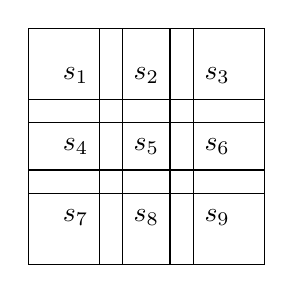
\begin{tikzpicture}[scale=0.9,
  cell/.style={draw, minimum size=12mm, inner sep=0pt}]
\node[cell] at (0,2) {$s_1$};
\node[cell] at (1,2) {$s_2$};
\node[cell] at (2,2) {$s_3$};
\node[cell] at (0,1) {$s_4$};
\node[cell] at (1,1) {$s_5$};
\node[cell] at (2,1) {$s_6$};
\node[cell] at (0,0) {$s_7$};
\node[cell] at (1,0) {$s_8$};
\node[cell] at (2,0) {$s_9$};
\end{tikzpicture}\\[2pt]
{(a) 状态}
\end{minipage}\hfill
% (b) 动作：含密集箭头示意，用源图
\begin{minipage}[b]{0.42\linewidth}
\centering
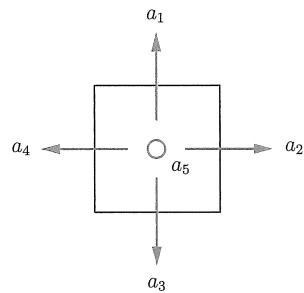
\includegraphics[width=\linewidth]{figures/rl/e6dcc00182df1a9da5b794a71a7549ecc67cb383d8f66d13f0926ec9367baa36.jpg}\\[2pt]
{(b) 动作}
\end{minipage}
\caption{状态和动作的示例。(a) 该网格有 $9$ 个状态：$\{s_1,s_2,\dots,s_9\}$。(b) 每个状态有 $5$ 个可能的动作：$\{a_1,a_2,a_3,a_4,a_5\}$。}
\label{fig:rl-basic-state-action}
\end{figure}

% ════════════════════════════════════════════════════════════════
\section{状态转移}
\label{sec:rl-basic-state-transition}

当执行一个动作时，智能体可能从一个状态转移到另一个状态，这样的过程被称为状态转移（state transition）。例如，如果智能体当前时刻处在状态 $s_1$ 并且执行动作 $a_2$（即向右移动），那么智能体会在下个时刻移动到状态 $s_2$，这个过程可以表示为
\begin{equation}
  s_1 \xrightarrow{a_2} s_2.
\end{equation}

下面我们考虑两个特殊但重要的情况。

当智能体试图越过网格世界的边界时，它下一个时刻应该转移到什么状态呢？例如，在状态 $s_1$ 采取动作 $a_1$（即向上移动）时，因为智能体不可能跳出状态空间，所以智能体会被弹回到某一个状态。这里我们设置智能体会被弹回到原来的状态，即 $s_1$。这样一个状态转移的过程可以表示为 $s_1 \xrightarrow{a_1} s_1$。

有的读者可能会问：智能体有没有可能被弹回到其他状态呢？答案是有可能的。因为这个网格世界是一个仿真环境，所以我们可以根据自己的喜好任意设置其状态转移过程。然而，如果是在现实世界中，那么状态转移需要服从物理规律，不再能任意设置。

当智能体试图进入禁止区域时，它下一个时刻应该转移到什么状态呢？例如，在状态 $s_5$ 采取动作 $a_2$（向右移动）。此时可能遇到两种情况。在第一种情况中，虽然 $s_6$ 是禁止区域，但它仍然是“可进入”的，只不过进入的时候会受到惩罚。此时，下一个状态是 $s_6$。这个状态转移的过程可以表示为 $s_5 \xrightarrow{a_2} s_6$。在第二种情况中，$s_6$ 是“不可进入”的，例如它四周被墙壁包围了起来。在这种情况下，智能体会被弹回到 $s_5$，此时的状态转移过程是 $s_5 \xrightarrow{a_2} s_5$。

我们究竟应该考虑哪种情况呢？因为这是一个仿真环境，所以我们可以随意选择。在本书中，我们选择第一种情况，即认为禁止区域仍然是可以进入的，只是智能体会受到惩罚。这种情况更为一般化并且更加有趣，例如之后我们会看到智能体可能会“冒险”穿过禁止区域，从而能更快地到达目标区域。

每一个状态的每一个动作都会对应一个状态转移过程。这些过程可以用一个表格来描述，如 \cref{tab:rl-basic-transition} 所示。在这个表格中，每一行对应一个状态，每一列对应一个动作。每个单元格给出了智能体会转移到的下一个状态。

\begin{table}[H]
\centering
\caption{状态转移过程可以用表格来表示。}
\label{tab:rl-basic-transition}
\begin{tabular}{cccccc}
\toprule
 & $a_1$（向上） & $a_2$（向右） & $a_3$（向下） & $a_4$（向左） & $a_5$（不动） \\
\midrule
$s_1$ & $s_1$ & $s_2$ & $s_4$ & $s_1$ & $s_1$ \\
$s_2$ & $s_2$ & $s_3$ & $s_5$ & $s_1$ & $s_2$ \\
$s_3$ & $s_3$ & $s_3$ & $s_6$ & $s_2$ & $s_3$ \\
$s_4$ & $s_1$ & $s_5$ & $s_7$ & $s_4$ & $s_4$ \\
$s_5$ & $s_2$ & $s_6$ & $s_8$ & $s_4$ & $s_5$ \\
$s_6$ & $s_3$ & $s_6$ & $s_9$ & $s_5$ & $s_6$ \\
$s_7$ & $s_4$ & $s_8$ & $s_7$ & $s_7$ & $s_7$ \\
$s_8$ & $s_5$ & $s_9$ & $s_8$ & $s_7$ & $s_8$ \\
$s_9$ & $s_6$ & $s_9$ & $s_9$ & $s_8$ & $s_9$ \\
\bottomrule
\end{tabular}
\end{table}

在数学上，状态转移过程可以通过条件概率来描述。例如，状态 $s_1$ 和动作 $a_2$ 对应的状态转移可以用如下条件概率描述：
\begin{equation}
\begin{aligned}
  & p(s_1 | s_1, a_2) = 0, \\
  & p(s_2 | s_1, a_2) = 1, \\
  & p(s_3 | s_1, a_2) = 0, \\
  & p(s_4 | s_1, a_2) = 0, \\
  & p(s_5 | s_1, a_2) = 0.
\end{aligned}
\end{equation}

该条件概率告诉我们：当在状态 $s_1$ 采取动作 $a_2$ 时，智能体转移到状态 $s_2$ 的概率是 $1$，而转移到其他任意状态的概率是 $0$。因此，在 $s_1$ 采取 $a_2$ 一定会导致智能体转移到 $s_2$。条件概率以及基本的概率知识可参阅相关概率论教材，供读者参考。

虽然直观，但是表格只能描述确定性的（deterministic）状态转移过程。其实状态转移也可以是随机性的（stochastic），此时需要用条件概率分布来描述。什么是随机性的状态转移过程呢？假设网格世界中有随机的阵风吹过。如果在状态 $s_1$ 采取动作 $a_2$，智能体可能被阵风吹到 $s_5$ 而不是 $s_2$。在这种情况下，我们有 $p(s_5 | s_1, a_2) > 0$，即下一个状态具有不确定性。不过简单起见，在本书网格世界的例子中，我们只考虑确定性的状态转移过程。

% ════════════════════════════════════════════════════════════════
\section{策略}
\label{sec:rl-basic-policy}

策略（policy）会告诉智能体在每一个状态应该采取什么样的动作。

在直观上，策略可以通过箭头来描述（\cref{fig:rl-basic-policy}(a)）。如果智能体执行某一个策略，那么它会从初始状态生成一条轨迹（\cref{fig:rl-basic-policy}(b)）。

\begin{figure}[ht]
\centering
\begin{minipage}[b]{0.46\linewidth}
\centering
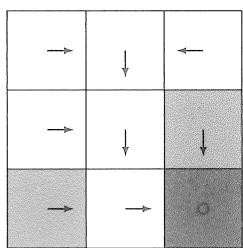
\includegraphics[width=\linewidth]{figures/rl/facda421bff6c50b141b153da76924cef50552813648b9f2a3aeb992bdf4d708.jpg}\\[2pt]
{(a) 一个确定性策略}
\end{minipage}\hfill
\begin{minipage}[b]{0.46\linewidth}
\centering
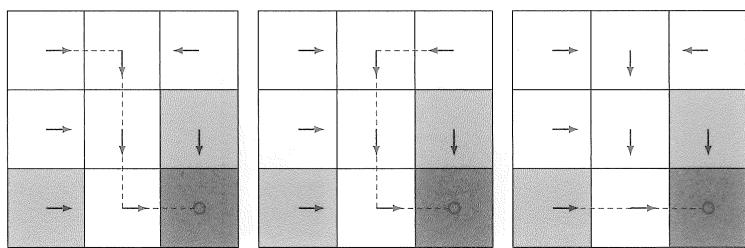
\includegraphics[width=\linewidth]{figures/rl/2368a305122a32d0e77e069aa7c8de24a85003d68d3c53fe967cd7fe3d703480.jpg}\\[2pt]
{(b) 从不同状态出发得到的轨迹}
\end{minipage}
\caption{一个确定性策略和对应的轨迹。}
\label{fig:rl-basic-policy}
\end{figure}

在数学上，策略可以通过条件概率来描述。我们常用 $\pi(a|s)$ 来表示在状态 $s$ 采取动作 $a$ 的概率（注意这里的 $\pi$ 不是圆周率）。这个概率对每一个状态和每一个动作都有定义。在 \cref{fig:rl-basic-policy} 所示的例子中，状态 $s_1$ 对应的策略是
\begin{equation}
\begin{aligned}
  & \pi(a_1 | s_1) = 0, \\
  & \pi(a_2 | s_1) = 1, \\
  & \pi(a_3 | s_1) = 0, \\
  & \pi(a_4 | s_1) = 0, \\
  & \pi(a_5 | s_1) = 0.
\end{aligned}
\end{equation}

该条件概率表明在状态 $s_1$ 采取动作 $a_2$ 的概率为 $1$，而采取其他任意动作的概率都为 $0$。其他状态 $\{s_2, s_3, \ldots, s_9\}$ 都可以用类似的条件概率来描述其对应的策略。

上面例子中的策略是确定性的。策略也可能是随机性的。例如，\cref{fig:rl-basic-stoch-policy} 中给出了一个随机策略：在状态 $s_1$，智能体有 $0.5$ 的概率采取向右的动作，有 $0.5$ 的概率采取向下的动作。此时在状态 $s_1$ 的策略是
\begin{equation}
\begin{aligned}
  & \pi(a_1 | s_1) = 0, \\
  & \pi(a_2 | s_1) = 0.5, \\
  & \pi(a_3 | s_1) = 0.5, \\
  & \pi(a_4 | s_1) = 0, \\
  & \pi(a_5 | s_1) = 0.
\end{aligned}
\end{equation}

\begin{figure}[ht]
\centering
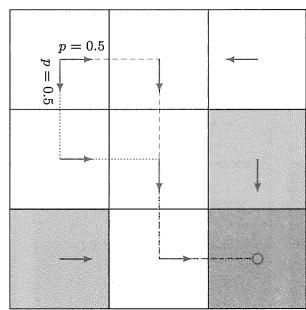
\includegraphics[width=0.5\linewidth]{figures/rl/40fbcc86242234aab3c879f1b9ba349f545c5fe3728332f48e191a6402887dd3.jpg}
\caption{一个随机性策略和对应的轨迹。在状态 $s_1$，智能体各有 $0.5$ 的概率向右或向下移动。}
\label{fig:rl-basic-stoch-policy}
\end{figure}

除了用条件概率，策略也可以用表格来描述。例如，\cref{tab:rl-basic-policy} 展示了 \cref{fig:rl-basic-stoch-policy} 中描绘的随机策略。其中第 $i$ 行和第 $j$ 列的元素对应了在第 $i$ 个状态采取第 $j$ 个动作的概率。这样的方法被称为表格表示法（tabular representation）。这种表格表示法是非常基础的，对于理解众多强化学习中的概念和算法至关重要。

\begin{table}[H]
\centering
\caption{用表格来表示一个策略。}
\label{tab:rl-basic-policy}
\begin{tabular}{cccccc}
\toprule
 & $a_1$（向上） & $a_2$（向右） & $a_3$（向下） & $a_4$（向左） & $a_5$（不动） \\
\midrule
$s_1$ & $0$ & $0.5$ & $0.5$ & $0$ & $0$ \\
$s_2$ & $0$ & $0$ & $1$ & $0$ & $0$ \\
$s_3$ & $0$ & $0$ & $0$ & $1$ & $0$ \\
$s_4$ & $0$ & $1$ & $0$ & $0$ & $0$ \\
$s_5$ & $0$ & $0$ & $1$ & $0$ & $0$ \\
$s_6$ & $0$ & $0$ & $1$ & $0$ & $0$ \\
$s_7$ & $0$ & $1$ & $0$ & $0$ & $0$ \\
$s_8$ & $0$ & $1$ & $0$ & $0$ & $0$ \\
$s_9$ & $0$ & $0$ & $0$ & $0$ & $1$ \\
\bottomrule
\end{tabular}
\end{table}

% ════════════════════════════════════════════════════════════════
\section{奖励}
\label{sec:rl-basic-reward}

奖励（reward）是强化学习中最独特的概念之一。

在一个状态执行一个动作后，智能体会获得奖励 $r$。$r$ 是一个实数，它是状态 $s$ 和动作 $a$ 的函数，可以写成 $r(s, a)$。其值可以是正数、负数或零。不同的奖励值对智能体最终学习到的策略有不同的影响。一般来说，正的奖励表示我们鼓励智能体采取相应的动作；负的奖励表示我们不鼓励智能体采取该动作。另外，如果 $r$ 是负数，此时称之为“惩罚”更为合适，不过我们一般不加区分地统一称之为“奖励”。

在之前提到的网格世界的例子中，我们可以设置如下奖励：
\begin{itemize}
  \item 如果智能体试图越过四周边界，设 $r_{\mathrm{boundary}} = -1$；
  \item 如果智能体试图进入禁止区域，设 $r_{\mathrm{forbidden}} = -1$；
  \item 如果智能体到达了目标区域，设 $r_{\mathrm{target}} = +1$；
  \item 在其他情况下，智能体获得的奖励为 $r_{\mathrm{other}} = 0$。
\end{itemize}

值得提醒读者的是，当智能体到达目标状态 $s_9$ 之后，它也许会持续执行策略，进而持续获得奖励。例如，如果智能体在 $s_9$ 采取动作 $a_5$（保持不动），下一个状态依然是 $s_9$，此时会继续获得奖励 $r_{\mathrm{target}} = +1$。如果智能体在 $s_9$ 执行动作 $a_2$（向右移动），会试图越过右侧边界，因此会被反弹回来，此时下一个状态也是 $s_9$，但奖励是 $r_{\mathrm{boundary}} = -1$。

奖励实际上是人机交互的一个重要手段：我们可以设置合适的奖励来引导智能体按照我们的预期来运动。例如，通过上述奖励设置，智能体会尽可能避免越过边界、避免进入禁止区域、力争进入目标区域。设计合适的奖励来实现我们的意图是强化学习中的一个重要环节。然而对于复杂的任务，这一环节可能并不简单，它需要用户能很好地理解所给定的任务。尽管如此，奖励的设计可能仍然比使用其他专业工具来设计策略更容易，这也是强化学习受众比较广的原因之一。

奖励的过程可以直观地表示为一个表格，如 \cref{tab:rl-basic-reward} 所示。表格的每一行对应一个状态，每一列对应一个动作。表格中每个单元格的值是在该状态采取该动作后可以获得的奖励。初学者可能会问一个问题：如果已知这个奖励表格，我们是否可以通过简单地选择对应最大奖励的动作来找到好的策略呢？答案是否定的。这是因为这些奖励只是即时奖励（immediate reward），即在采取一个动作后可以立刻获得的奖励。如果要寻找一个好的策略，那么必须考虑更长远的总奖励（total reward）（更多信息将在 \cref{sec:rl-basic-trajectory} 中给出）。具有最大即时奖励的动作不一定能带来最大的总奖励。

\begin{table}[H]
\centering
\caption{奖励可以用表格来表示。}
\label{tab:rl-basic-reward}
\begin{tabular}{cccccc}
\toprule
 & $a_1$（向上） & $a_2$（向右） & $a_3$（向下） & $a_4$（向左） & $a_5$（不动） \\
\midrule
$s_1$ & $r_{\mathrm{boundary}}$ & $0$ & $0$ & $r_{\mathrm{boundary}}$ & $0$ \\
$s_2$ & $r_{\mathrm{boundary}}$ & $0$ & $0$ & $0$ & $0$ \\
$s_3$ & $r_{\mathrm{boundary}}$ & $r_{\mathrm{boundary}}$ & $r_{\mathrm{forbidden}}$ & $0$ & $0$ \\
$s_4$ & $0$ & $0$ & $r_{\mathrm{forbidden}}$ & $r_{\mathrm{boundary}}$ & $0$ \\
$s_5$ & $0$ & $r_{\mathrm{forbidden}}$ & $0$ & $0$ & $0$ \\
$s_6$ & $0$ & $r_{\mathrm{boundary}}$ & $r_{\mathrm{target}}$ & $0$ & $r_{\mathrm{forbidden}}$ \\
$s_7$ & $0$ & $0$ & $r_{\mathrm{boundary}}$ & $r_{\mathrm{boundary}}$ & $r_{\mathrm{forbidden}}$ \\
$s_8$ & $0$ & $r_{\mathrm{target}}$ & $r_{\mathrm{boundary}}$ & $r_{\mathrm{forbidden}}$ & $0$ \\
$s_9$ & $r_{\mathrm{forbidden}}$ & $r_{\mathrm{boundary}}$ & $r_{\mathrm{boundary}}$ & $0$ & $r_{\mathrm{target}}$ \\
\bottomrule
\end{tabular}
\end{table}

虽然直观，但是表格表示只能描述确定性的奖励过程。为了描述更加一般化的奖励过程，我们可以使用条件概率：$p(r|s,a)$ 表示在状态 $s$ 采取动作 $a$ 得到奖励 $r$ 的概率。在前述的例子中，对状态 $s_1$，有
\begin{equation}
  p(r = -1 | s_1, a_1) = 1, \quad p(r \neq -1 | s_1, a_1) = 0.
\end{equation}

该条件概率表明在 $s_1$ 采取 $a_1$ 得到 $r = -1$ 的概率是 $1$，而得到任何其他奖励值的概率是 $0$。这个奖励是确定性的，因此既可以用表格也可以用条件概率来描述。然而，如果奖励过程是随机的，那么表格法将不再适用，而只能使用条件概率。例如，$p(r = -1|s_1, a_1) = 0.5$，$p(r = -2|s_1, a_1) = 0.5$，即各有 $0.5$ 的概率获得 $-1$ 或者 $-2$ 的奖励。值得强调的是，本书中的网格世界的例子都只考虑确定性的奖励过程。这里只给出一个简单的例子，读者可以感受一下为什么奖励可能是随机的。例如，如果一个学生努力学习，他或她一般会得到正面的奖励（例如考试成绩好），不过奖励的具体数值（例如考试成绩）可能是不确定的，可能是 $100$ 分，也可能是 $90$ 分，这个过程受到了很多因素的影响。

% ════════════════════════════════════════════════════════════════
\section{轨迹、回报、回合}
\label{sec:rl-basic-trajectory}

一条轨迹（trajectory）指的是一个“状态-动作-奖励”的链条。例如，根据 \cref{fig:rl-basic-two-policies}(a) 所示的策略，智能体从 $s_1$ 出发会得到如下轨迹：
\begin{equation}
  s_1 \xrightarrow[r=0]{a_2} s_2 \xrightarrow[r=0]{a_3} s_5 \xrightarrow[r=0]{a_3} s_8 \xrightarrow[r=1]{a_2} s_9.
\end{equation}

沿着一条轨迹，智能体会得到一系列的即时奖励，这些即时奖励之和被称为回报（return）。例如，上述轨迹对应的回报是
\begin{equation}
  \mathrm{return} = 0 + 0 + 0 + 1 = 1. \label{eq:rl-basic-return1}
\end{equation}

回报由即时奖励（immediate reward）和未来奖励（future reward）组成。这里，即时奖励是在初始状态执行动作后立刻获得的奖励；未来奖励指的是离开初始状态后获得的奖励之和。例如，上述轨迹对应的即时奖励是 $0$，但是未来奖励是 $1$，因此总奖励是 $1$。另外，回报也可以被称为总奖励（total reward）或累积奖励（cumulative reward）。

\begin{figure}[ht]
\centering
\begin{minipage}[b]{0.46\linewidth}
\centering
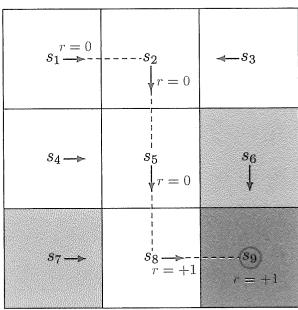
\includegraphics[width=\linewidth]{figures/rl/a9c64fa4308103eee93f7e31a4ca7439a819e723430113b0ba6d57a219a52e7a.jpg}\\[2pt]
{(a) 策略 1 及其轨迹}
\end{minipage}\hfill
\begin{minipage}[b]{0.46\linewidth}
\centering
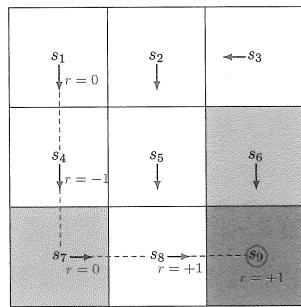
\includegraphics[width=\linewidth]{figures/rl/720b962add2493c709396e3c53dabfc06a1f1586c31dd50f075f3ab4cfb2bd2e.jpg}\\[2pt]
{(b) 策略 2 及其轨迹}
\end{minipage}
\caption{两种策略及其对应的轨迹。}
\label{fig:rl-basic-two-policies}
\end{figure}

回报可以用于评价一个策略的“好坏”。例如，对于 \cref{fig:rl-basic-two-policies} 中的两个策略，我们可以分别计算两条轨迹对应的回报，进而判断哪个策略更好。具体来说，如果按照 \cref{fig:rl-basic-two-policies} 中左边的策略，从 $s_1$ 开始所获得的回报等于 $1$，计算过程已经在 \cref{eq:rl-basic-return1} 中给出。如果按照 \cref{fig:rl-basic-two-policies} 中右边的策略，从 $s_1$ 开始则得到如下轨迹：
\begin{equation}
  s_1 \xrightarrow[r=0]{a_3} s_4 \xrightarrow[r=-1]{a_3} s_7 \xrightarrow[r=0]{a_2} s_8 \xrightarrow[r=+1]{a_2} s_9.
\end{equation}

相应的回报为
\begin{equation}
  \mathrm{return} = 0 - 1 + 0 + 1 = 0. \label{eq:rl-basic-return2}
\end{equation}

根据 \cref{eq:rl-basic-return1} 和 \cref{eq:rl-basic-return2} 计算得到的回报，我们知道左边的策略相比右边的策略能得到更大的回报，因此也更好。这个数学结论与我们的直觉是一致的：右侧的策略更差，因为它会经过禁止区域。关于策略的好坏以及评价，我们将在 \cref{ch:rl-bellman} 和 \cref{ch:rl-bellman-opt} 进行详细介绍。

刚刚我们提到的轨迹都是有限长的，实际上轨迹也可以无限长。例如，\cref{fig:rl-basic-two-policies} 中的轨迹在到达 $s_9$ 后可能并不会停止，而是继续执行策略。具体来说，这里的策略是在到达 $s_9$ 后保持不动，因此智能体会不断得到 $+1$ 的奖励，所对应的轨迹也是无限长的：
\begin{equation}
  s_1 \xrightarrow[r=0]{a_2} s_2 \xrightarrow[r=0]{a_3} s_5 \xrightarrow[r=0]{a_3} s_8 \xrightarrow[r=1]{a_2} s_9 \xrightarrow[r=1]{a_5} s_9 \xrightarrow[r=1]{a_5} s_9 \dots
\end{equation}

此时，如果我们直接把这条轨迹上所有的奖励求和来计算回报，那么得到的是
\begin{equation}
  \mathrm{return} = 0 + 0 + 0 + 1 + 1 + 1 + \dots = \infty.
\end{equation}

这里因为轨迹是无限长的，所以计算的回报会发散到无穷。此时，我们需要引入折扣回报（discounted return）的概念。令 $\gamma \in (0,1)$ 为折扣因子（discount rate）。折扣回报是所有折扣奖励的总和，即为不同时刻得到的奖励添加相应的折扣再求和：
\begin{equation}
  \mathrm{discounted\ return} = 0 + \gamma 0 + \gamma^2 0 + \gamma^3 1 + \gamma^4 1 + \gamma^5 1 + \dots \label{eq:rl-basic-discounted}
\end{equation}

由于 $\gamma \in (0,1)$，\cref{eq:rl-basic-discounted} 中的折扣回报的值不再是无穷了，而是一个有限值：
\begin{equation}
  \mathrm{discounted\ return} = \gamma^3 (1 + \gamma + \gamma^2 + \dots) = \gamma^3 \frac{1}{1 - \gamma}.
\end{equation}

折扣因子的引入具有以下用途。第一，它允许考虑无限长的轨迹，而不用担心回报会发散到无穷；第二，折扣因子可以用来调整对近期或远期奖励的重视程度。具体来说，如果 $\gamma$ 接近 $0$，则智能体会更加重视近期奖励，最后所得到的策略也会比较短视。如果 $\gamma$ 接近 $1$，则智能体会更加重视远期奖励，最后所得到的策略也会更具有远见，例如敢于冒险在近期获得负面奖励来获得更大的未来奖励。这些结论将在后续关于贝尔曼最优性的章节通过例子详细展示。

当执行一个策略进而与环境交互时，智能体从初始状态开始到终止状态（terminal state）停止的过程被称为一个回合（episode）或尝试（trial）。这里的 Episode 有多种翻译，例如回合、情节、集、轮等，其中“回合”能比较好地描述其内涵。不过，它应该与神经网络训练过程中的回合（epoch）加以区分。

回合和轨迹在概念上非常类似：回合通常被认为是一条有限长的轨迹。如果一个任务最多有有限步，那么这样的任务称为回合制任务（episodic task）。如果一个任务没有终止状态，则意味着智能体与环境的交互永不停止，这种任务被称为持续性任务（continuing task）。为了在数学上可以不加区分地对待这两种任务，我们可以把回合制任务转换为持续性任务。为此，我们只需要合理定义智能体在到达终止状态后的状态和动作等元素即可。具体来说，在回合制任务中到达终止状态后，我们有如下两种方式将其转换为持续性任务。

第一，我们可以将终止状态视为一个特殊状态，即专门设计其动作空间或状态转移，从而使智能体永远停留在此状态，这样的状态被称为吸收状态（absorbing state），即一旦达到这样的状态就会一直停留在该状态。例如，对于目标状态 $s_9$，我们可以指定其动作空间为 $\mathcal{A}(s_9) = \{a_5\}$，即到达这个状态后唯一可执行的动作就是原地不动。

第二，我们可以将终止状态视为一个普通状态，即将其与其他状态一视同仁，此时智能体可能会离开该状态并再次回来。由于每次到达 $s_9$ 都可以获得 $r = 1$ 的正奖励，可以预期的是智能体最终会学会永远停留在 $s_9$ 以获得更多的奖励。值得注意的是，将回合制任务转换为持续性任务需要使用折扣因子，以避免回报趋于无穷。

本书将考虑第二种情况，即将目标状态视为一个普通状态，其动作空间为 $\mathcal{A} = \{a_1, a_2, \ldots, a_5\}$。由于智能体到达这个状态之后仍然允许离开这个状态，因此这是一种更加一般化的情况，我们需要让智能体学习到在到达这个状态之后能够保持原地不动。

% ════════════════════════════════════════════════════════════════
\section{马尔可夫决策过程}
\label{sec:rl-basic-mdp}

前面几节通过例子直观地介绍了强化学习中的基本概念。本节将在马尔可夫决策过程（Markov decision process, MDP）的框架下以更加正式的方式介绍这些概念。

马尔可夫决策过程是描述随机动态系统的一般框架，它并不局限于强化学习，而是强化学习需要依赖于这个框架。马尔可夫决策过程涉及以下关键要素。

\begin{itemize}
  \item 集合：
  \begin{itemize}
    \item 状态空间：所有状态的集合，记为 $\mathcal{S}$。
    \item 动作空间：与每个状态 $s \in \mathcal{S}$ 相关联的所有动作的集合，记为 $\mathcal{A}(s)$。
    \item 奖励集合：与 $(s, a)$ 相关联的所有奖励的集合，记为 $\mathcal{R}(s, a)$。
  \end{itemize}
  \item 模型：
  \begin{itemize}
    \item 状态转移概率：在状态 $s$ 采取动作 $a$ 时，智能体转移到状态 $s'$ 的概率为 $p(s'|s,a)$。对于任意 $(s,a)$，都有 $\sum_{s' \in \mathcal{S}} p(s'|s,a) = 1$。
    \item 奖励概率：在状态 $s$ 采取动作 $a$ 时，智能体获得奖励 $r$ 的概率是 $p(r|s,a)$。对于任意 $(s,a)$，都有 $\sum_{r \in \mathcal{R}(s,a)} p(r|s,a) = 1$ 成立。
  \end{itemize}
  \item 策略：在状态 $s$，智能体采取动作 $a$ 的概率是 $\pi(a|s)$。对于任意 $s \in \mathcal{S}$，都有 $\sum_{a \in \mathcal{A}(s)} \pi(a|s) = 1$。
  \item 马尔可夫性质：马尔可夫性质（Markov property）指的是随机过程中的无记忆性质，它在数学上表示为
\begin{equation}
\begin{aligned}
  & p(s_{t+1} | s_t, a_t, s_{t-1}, a_{t-1}, \ldots, s_0, a_0) = p(s_{t+1} | s_t, a_t), \\
  & p(r_{t+1} | s_t, a_t, s_{t-1}, a_{t-1}, \ldots, s_0, a_0) = p(r_{t+1} | s_t, a_t),
\end{aligned}
\label{eq:rl-basic-markov}
\end{equation}
  其中 $t$ 表示当前时刻，$t+1$ 表示下一个时刻。\cref{eq:rl-basic-markov} 表示下一个状态和奖励仅依赖于当前时刻的状态和动作，而与之前时刻的状态和动作无关。
\end{itemize}

在马尔可夫决策过程中，$p(s'|s,a)$ 和 $p(r|s,a)$ 被称为模型（model）或者动态（dynamics）。模型可以是平稳的（stationary）或非平稳的（nonstationary）：平稳模型不会随时间变化，而非平稳模型会随时间变化。例如，在网格世界例子中，如果一个禁区时而出现时而消失，那么所对应的状态转移或者奖励就会随时间变化，此时系统是非平稳的。本书只考虑平稳的情况。

读者可能还听说过马尔可夫过程（Markov process, MP）。那么“马尔可夫过程”与“马尔可夫决策过程”有什么区别与联系呢？答案很简单：一旦在马尔可夫决策过程中的策略确定下来了，马尔可夫决策过程就退化成了一个马尔可夫过程。例如，\cref{fig:rl-basic-mp} 中网格世界的策略已经给定，此时整个系统可以被抽象为一个马尔可夫过程。最后，本书主要考虑有限的马尔可夫决策过程，即状态和动作的数量都是有限的。初学者应该首先透彻地理解这一最简单的情况，再学习更加复杂的情况。

\begin{figure}[ht]
\centering
% （左图）给定策略的网格世界：箭头代表策略；s1 为随机策略（0.5 向右、0.5 向下）
\begin{minipage}[b]{0.40\linewidth}
\centering
\begin{tikzpicture}[scale=0.78, >=Stealth,
  cell/.style={draw, minimum size=14mm, inner sep=0pt},
  forb/.style={cell, fill=second!22},
  targ/.style={cell, fill=main!18},
  pol/.style={->, thick}]
% 3x3 网格（禁止区 s6/s7，目标 s9）
\foreach \x in {0,1,2}{\foreach \y in {0,1,2}{\node[cell] at (\x,\y) {};}}
\node[forb] at (2,1) {};
\node[forb] at (0,0) {};
\node[targ] at (2,0) {};
% 策略箭头：s1 随机（向右 0.5、向下 0.5）
\draw[pol] (-0.15,2.15) -- (0.35,2.15) node[midway,above,font=\tiny]{$p=0.5$};
\draw[pol] (-0.2,2.05) -- (-0.2,1.55) node[midway,left,font=\tiny]{$p=0.5$};
% 其余状态确定性策略
\draw[pol] (1,2) -- (1,1.55);   % s2 向下
\draw[pol] (2,2) -- (1.6,2);    % s3 向左
\draw[pol] (0,1) -- (0.45,1);   % s4 向右
\draw[pol] (1,1) -- (1,0.55);   % s5 向下
\draw[pol] (2,1) -- (2,0.55);   % s6 向下
\draw[pol] (0,0) -- (0.45,0);   % s7 向右
\draw[pol] (1,0) -- (1.55,0);   % s8 向右
\draw[pol] (2,0) ++(0.18,0.18) arc (-60:240:0.18); % s9 原地不动（自环）
\end{tikzpicture}
\end{minipage}\hfill
% （右图）抽象出的马尔可夫过程：圆圈=状态，箭头=状态转移，标注 Prob
\begin{minipage}[b]{0.56\linewidth}
\centering
\begin{tikzpicture}[scale=0.85, >=Stealth,
  st/.style={circle, draw, minimum size=8mm, inner sep=0pt, font=\small, fill=main!10},
  ln/.style={->, thick, gray!55!black},
  pl/.style={font=\tiny, midway}]
% 3x3 状态圆圈阵列
\foreach \i/\x/\y in {1/0/2, 2/1.7/2, 3/3.4/2, 4/0/1, 5/1.7/1, 6/3.4/1, 7/0/0, 8/1.7/0, 9/3.4/0}{
  \node[st] (n\i) at (\x,\y) {$s_{\i}$};
}
% 给定（随机）策略下的转移，每条箭头标注转移概率
\draw[ln] (n1)--(n2) node[pl,above]{Prob=0.5};
\draw[ln] (n1)--(n4) node[pl,left]{Prob=0.5};
\draw[ln] (n3)--(n2) node[pl,above]{Prob=1};
\draw[ln] (n2)--(n5) node[pl,right]{Prob=1};
\draw[ln] (n4)--(n5) node[pl,below]{Prob=1};
\draw[ln] (n5)--(n8) node[pl,right]{Prob=1};
\draw[ln] (n6)--(n9) node[pl,right]{Prob=1};
\draw[ln] (n7)--(n8) node[pl,below]{Prob=1};
\draw[ln] (n8)--(n9) node[pl,below]{Prob=1};
\draw[ln] (n9) to[out=-30,in=30,looseness=6] (n9) node[pl,right]{Prob=1};  % s9 自环（原地不动）
\end{tikzpicture}
\end{minipage}
\caption{将一个网格世界的例子抽象成马尔可夫过程。右图中的圆圈代表状态，箭头代表状态转移。}
\label{fig:rl-basic-mp}
\end{figure}

强化学习的过程涉及智能体与环境的交互，智能体之外的一切都被视为环境（environment）。第一，智能体是一个感知者，例如具有眼睛能够感知并理解当前的状态；第二，智能体是一个决策者，例如具有大脑能够做出决策，知道在什么状态应该采取什么行动；第三，智能体是一个执行者，例如具有操作机构来执行策略所指示的动作，从而改变状态并得到奖励。

% ════════════════════════════════════════════════════════════════
\section{总结}
\label{sec:rl-basic-summary}

本章介绍了强化学习中的基本概念，这些概念将在本书后面广为使用。我们首先使用网格世界的例子来直观地介绍这些概念，进而在马尔可夫决策过程的框架中对它们进行了正式的介绍。关于马尔可夫决策过程的更多信息，读者可以参考强化学习与马尔可夫决策过程方面的经典著作。

% ════════════════════════════════════════════════════════════════
\section{问答}
\label{sec:rl-basic-qa}

\textbf{提问：奖励为正数一定代表鼓励，奖励为负数一定代表惩罚吗？}

回答：本章提到正奖励会鼓励智能体采取相应动作，而负奖励会鼓励智能体不要采取相应动作。知道这一点对于初学者已经足够了。不过，这种说法并不严谨。

严格来说，是奖励的相对值而不是绝对值决定了鼓励或惩罚。例如，这一章设定了 $r_{\mathrm{boundary}} = -1$，$r_{\mathrm{forbidden}} = -1$，$r_{\mathrm{target}} = +1$，$r_{\mathrm{other}} = 0$。我们也可以在这些值加上一个常数而不改变最终的最优策略，例如给所有奖励加上 $-2$ 从而得到 $r_{\mathrm{boundary}} = -3$，$r_{\mathrm{forbidden}} = -3$，$r_{\mathrm{target}} = -1$，$r_{\mathrm{other}} = -2$。虽然此时的奖励都是负数，但最终的最优策略仍然不变。从直观上来说，由于 $r_{\mathrm{target}} = -1$ 相比 $r_{\mathrm{forbidden}} = -3$ 惩罚得更少，因此 $r_{\mathrm{target}} = -1$ 已经算是鼓励了。这里就不展开介绍细节了，更多信息可以参见后续关于贝尔曼最优性的章节中关于奖励仿射变换不变性的讨论。

\medskip
\textbf{提问：奖励是下一个状态的函数吗？}

回答：本章提到了奖励 $r$ 是状态 $s$ 和动作 $a$ 的函数，但是并没有提及 $r$ 是下一个状态 $s'$ 的函数。从直观上来说，下一个状态是与奖励息息相关的。例如，当下一个状态是目标区域时，通常设置奖励为正数；当下一个状态是禁止区域时，通常设置奖励为负数。那么一个自然的问题是：奖励是否是下一个状态的函数？这个问题的数学描述是：我们是否应该使用 $p(r|s,a,s')$（其中 $s'$ 代表下一个状态）而不是 $p(r|s,a)$？这个问题的答案是：$r$ 实际上依赖于 $s$、$a$、$s'$ 这三者。然而，因为 $s'$ 也依赖于 $s$ 和 $a$，所以我们可以等效地将 $r$ 写为 $s$ 和 $a$ 的函数：$p(r|s,a) = \sum_{s'} p(r|s,a,s') p(s'|s,a)$。通过这种方式，我们在 \cref{ch:rl-bellman} 中可以轻易地建立起贝尔曼方程。
